\chapter{Конструкторская часть}

В этой части будут представлены схемы разработанных алгоритмов.

\section{Схемы алгоритмов}

\subsection{Последовательного алгоритм}

На рисунке~\ref{img:sequential} приведена схема последовательного алгоритма по поиску пар вершин, находящихся на расстоянии меньше заданного.

На рисунке~\ref{img:min_dist_matrix} приведена схема алгоритма создания матрицы минимальных расстояний из матрицы смежности.

На рисунке~\ref{img:choose_pairs} приведена схема алгоритма выбора пар вершин на расстоянии меньше заданного из матрицы минимальных расстояний.

\begin{figure}[H]
	\centering
	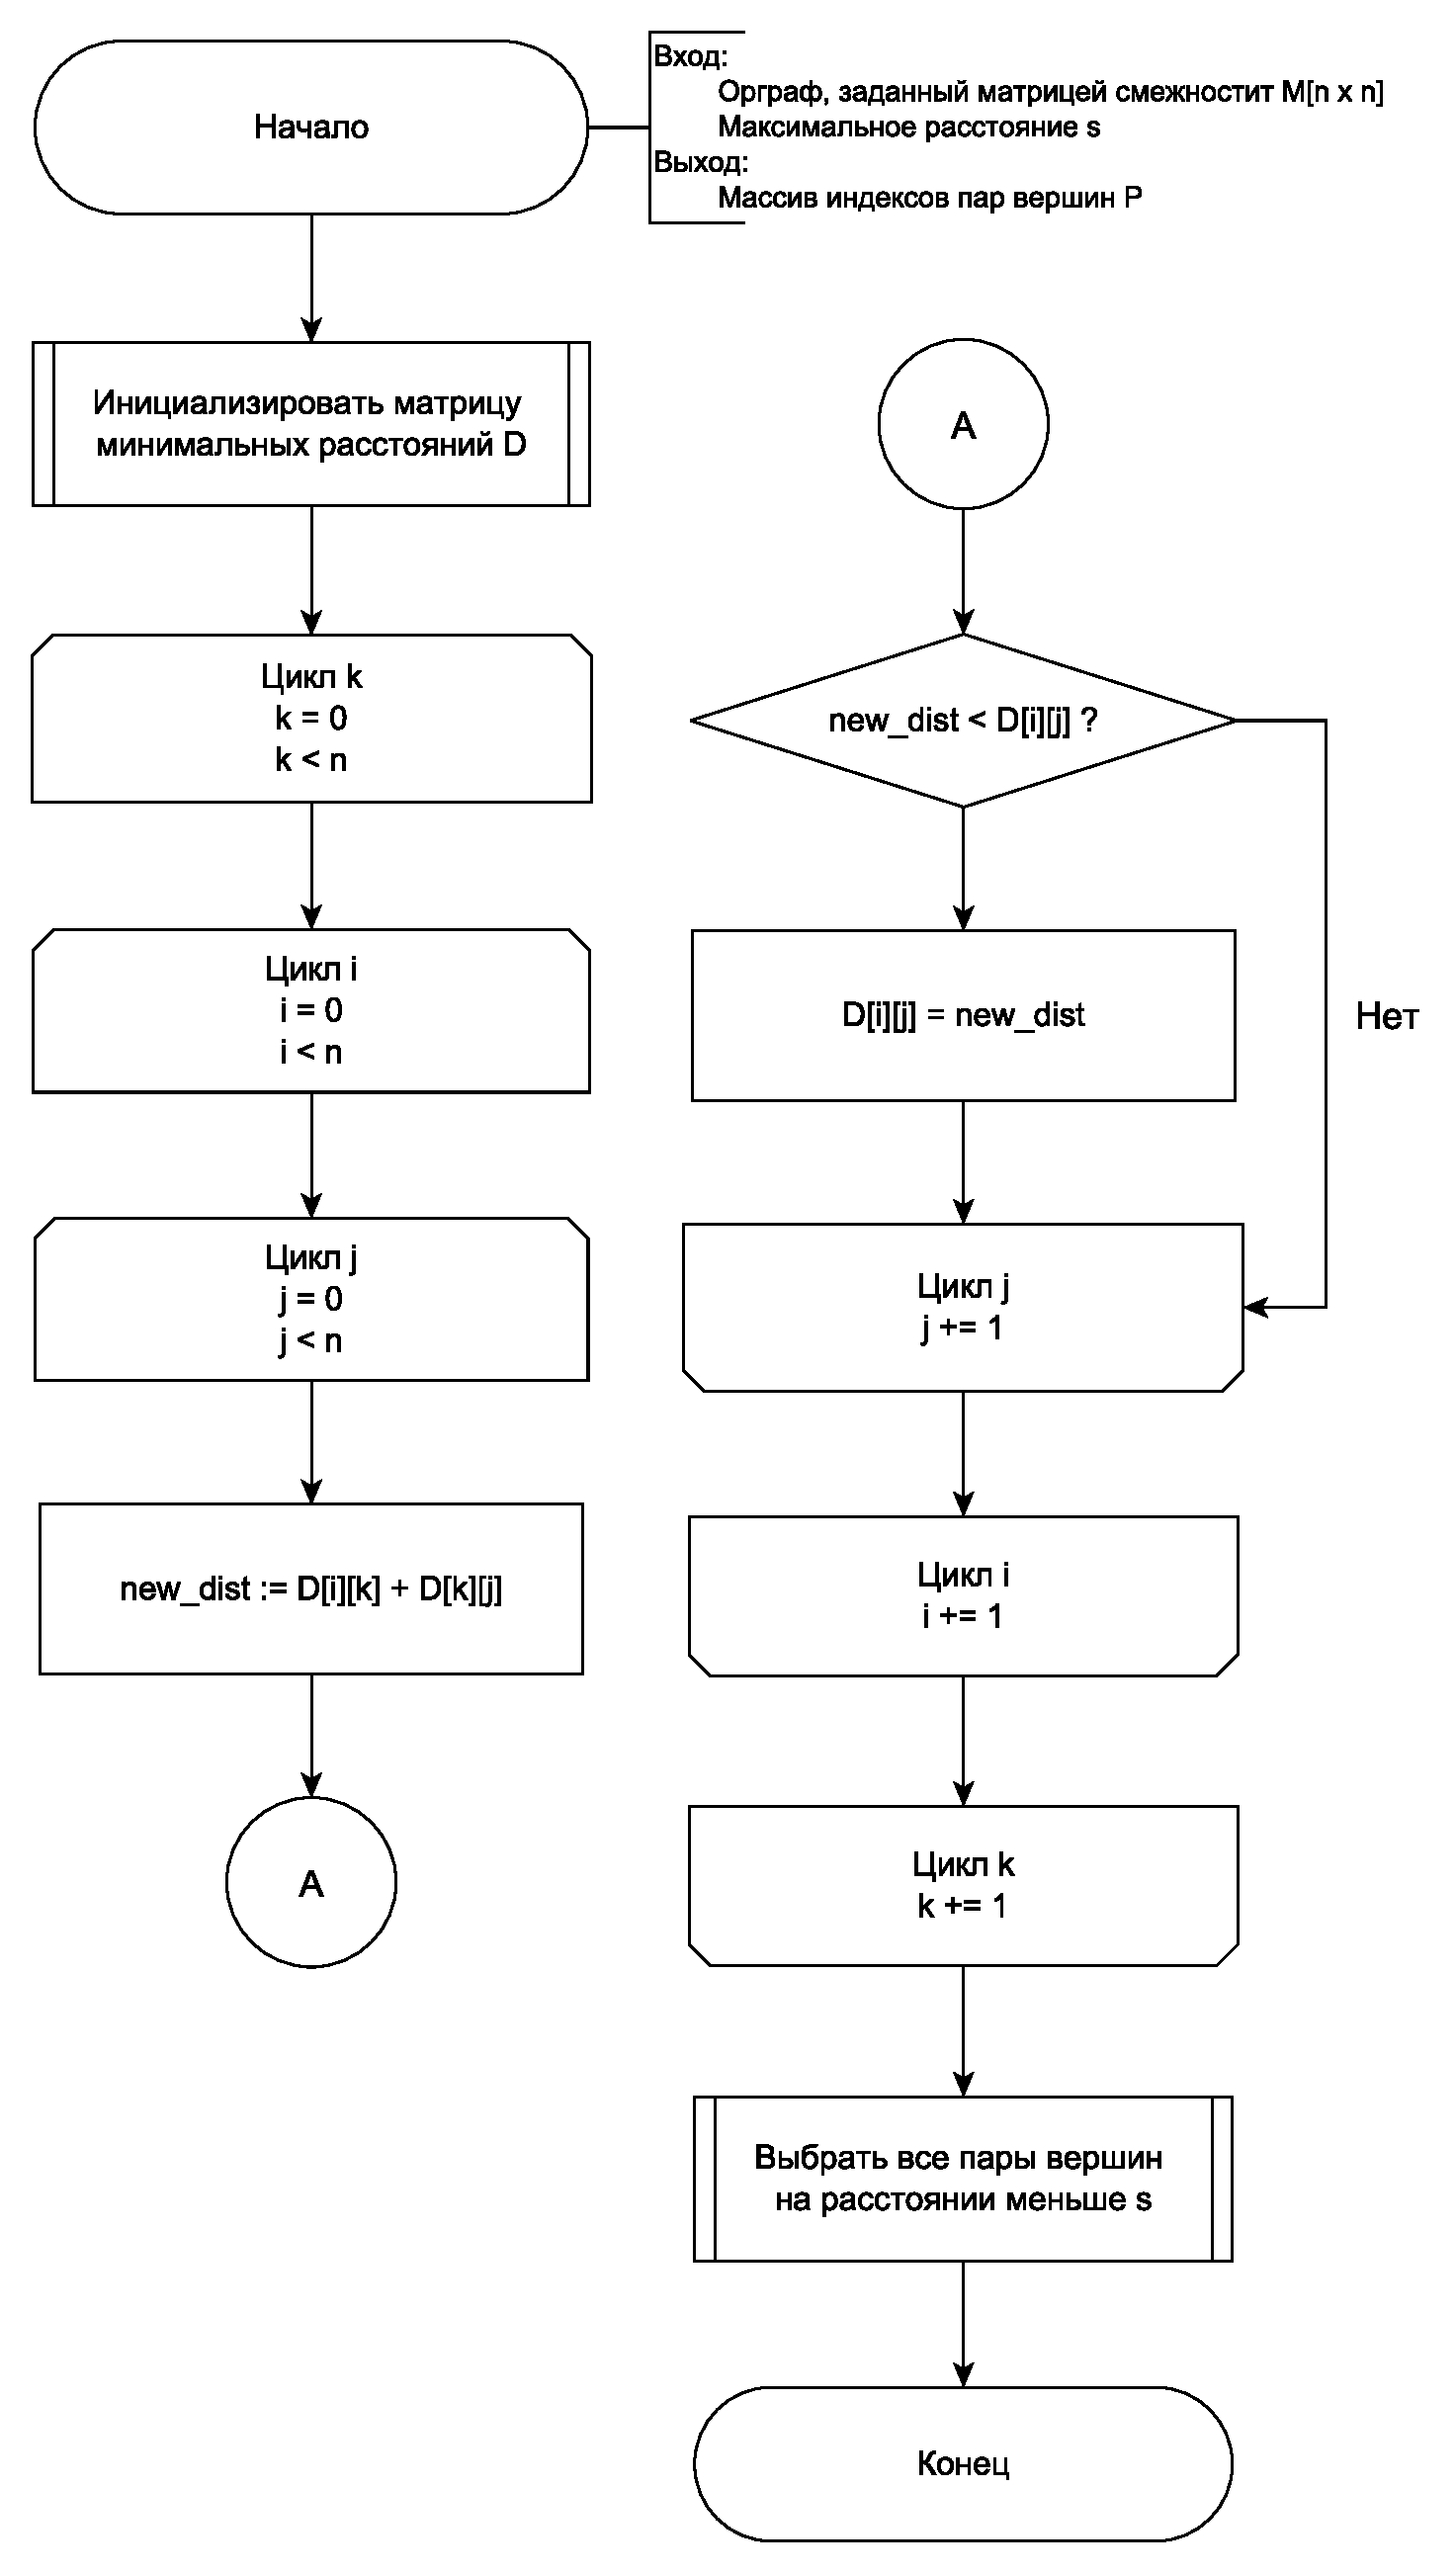
\includegraphics[height=0.6\textheight]{images/sequential.pdf}
	\caption{Схема последовательного алгоритма}
	\label{img:sequential}
\end{figure}

\begin{figure}[H]
	\centering
	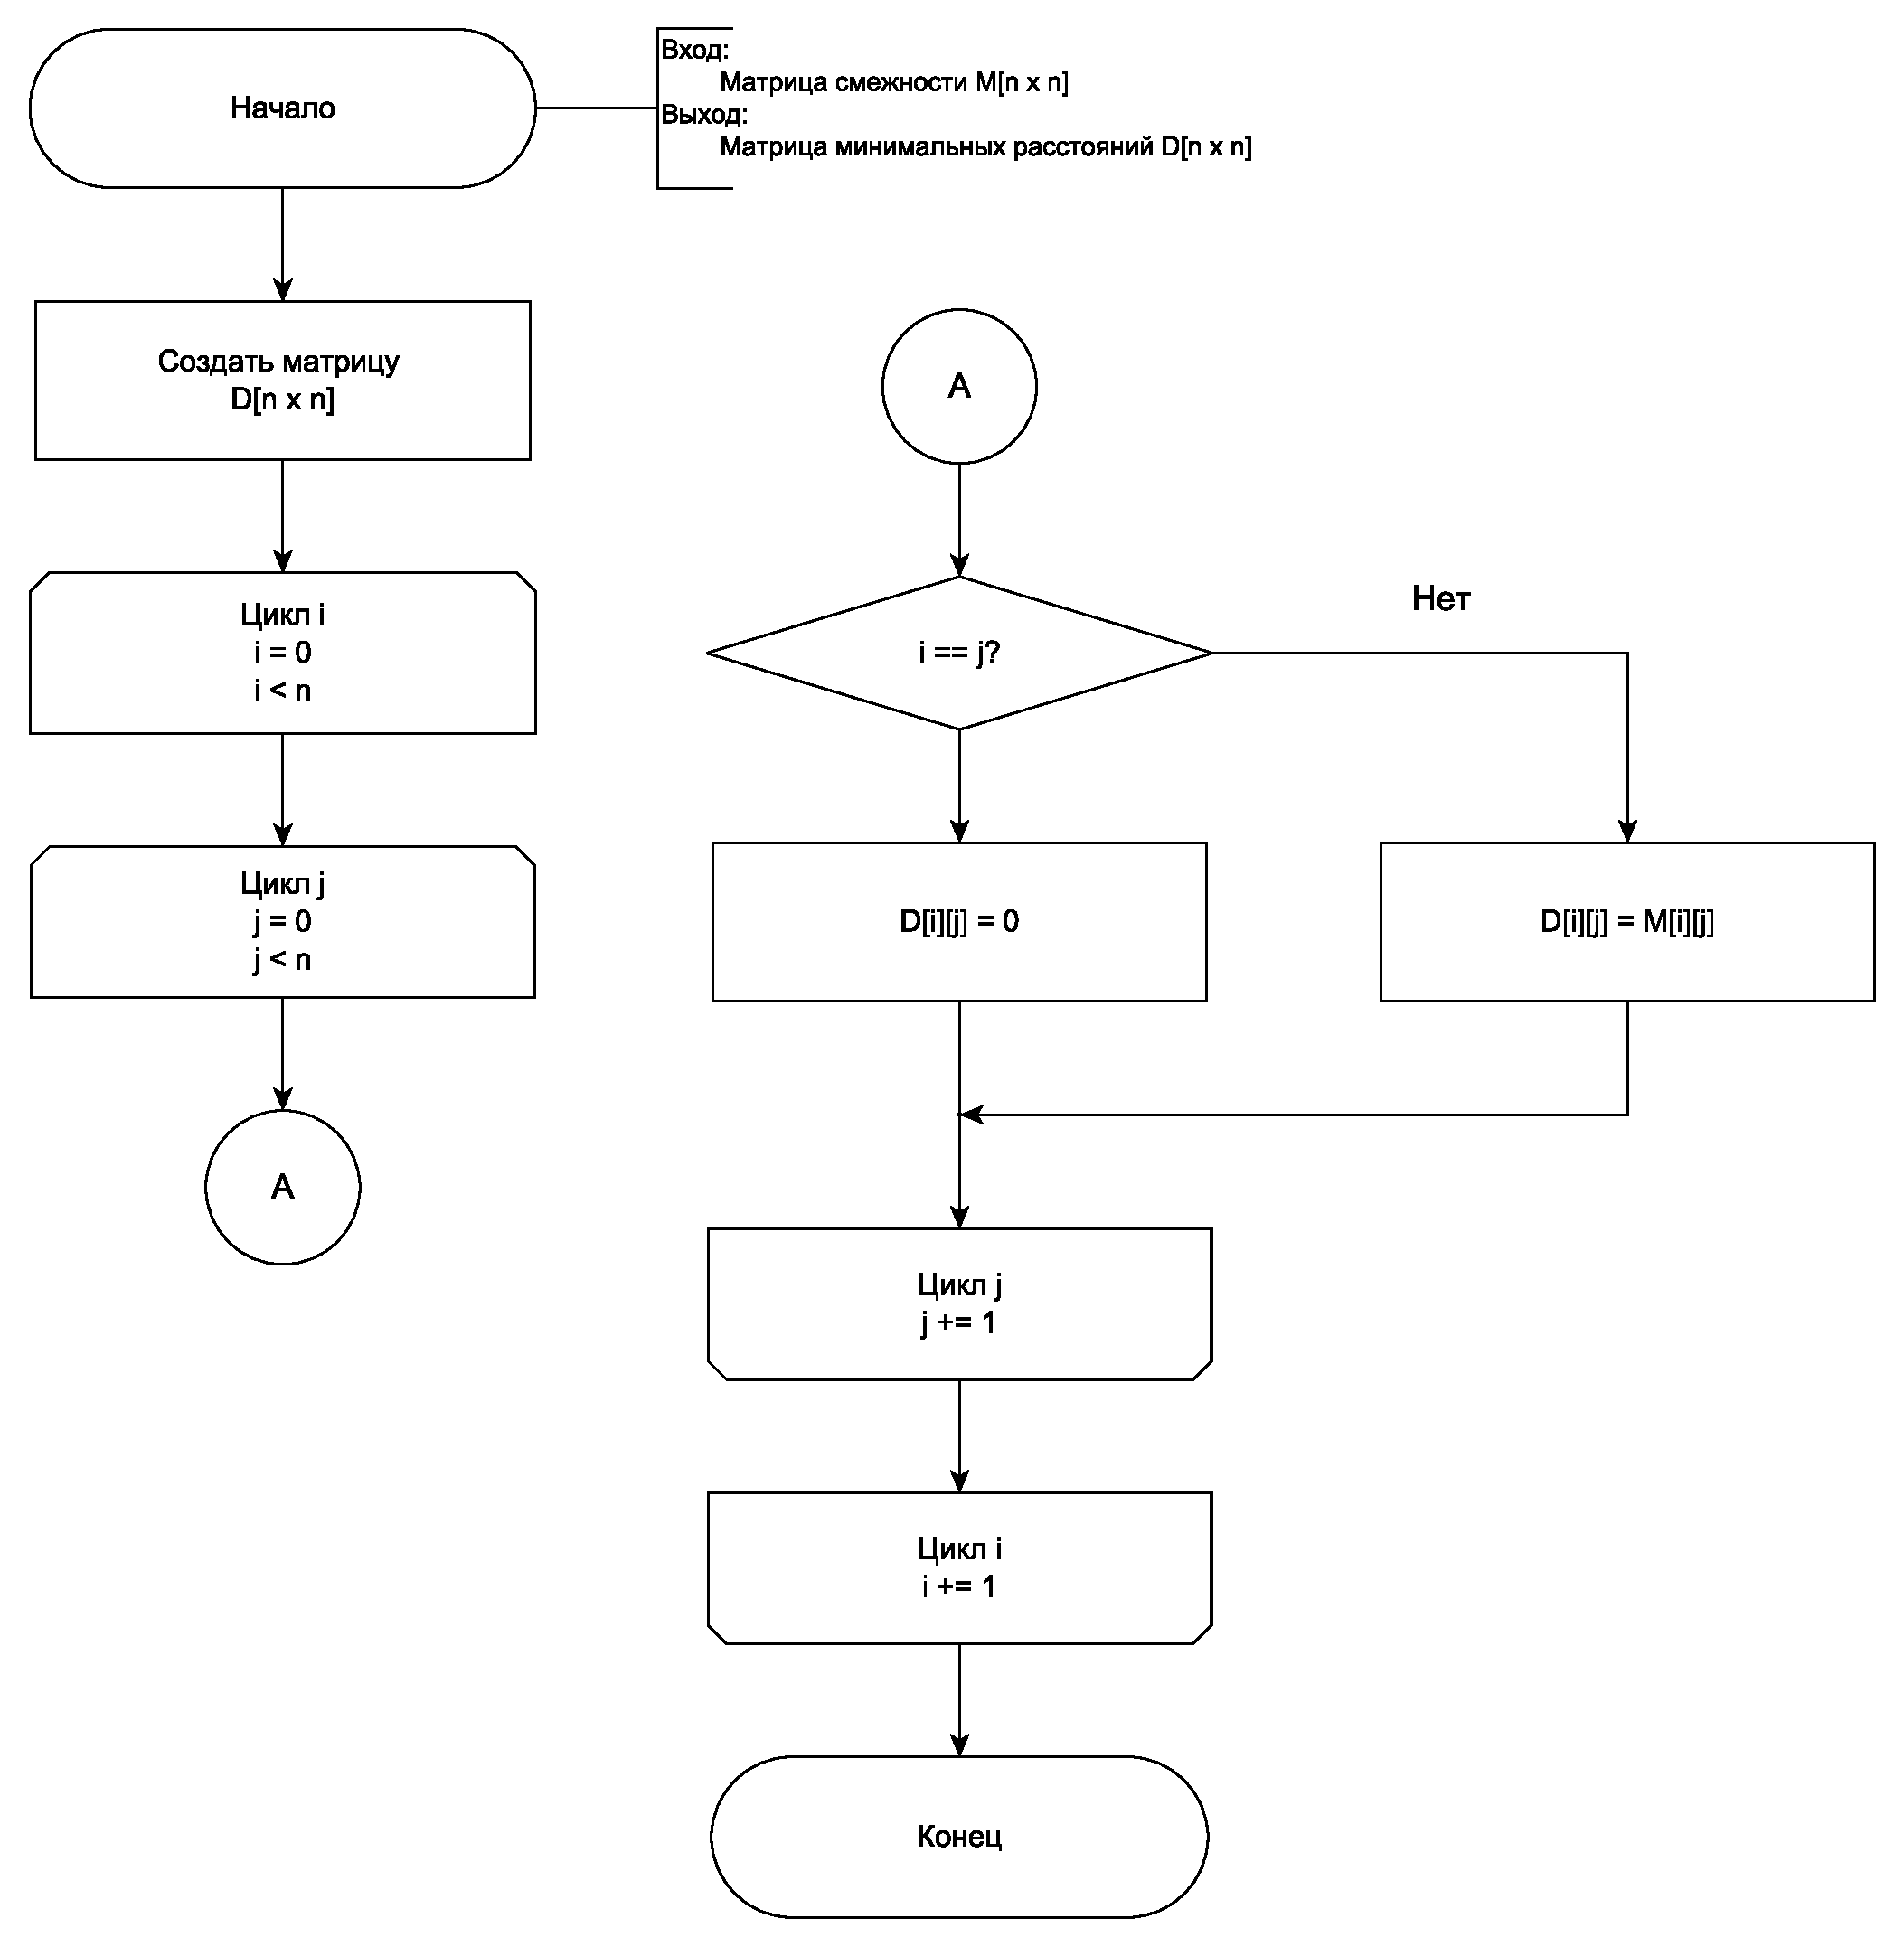
\includegraphics[width=1\textwidth]{images/min_dist_matrix.pdf}
	\caption{Схема алгоритма инициализации матрицы кратчайших расстояний}
	\label{img:min_dist_matrix}
\end{figure}

\begin{figure}[H]
	\centering
	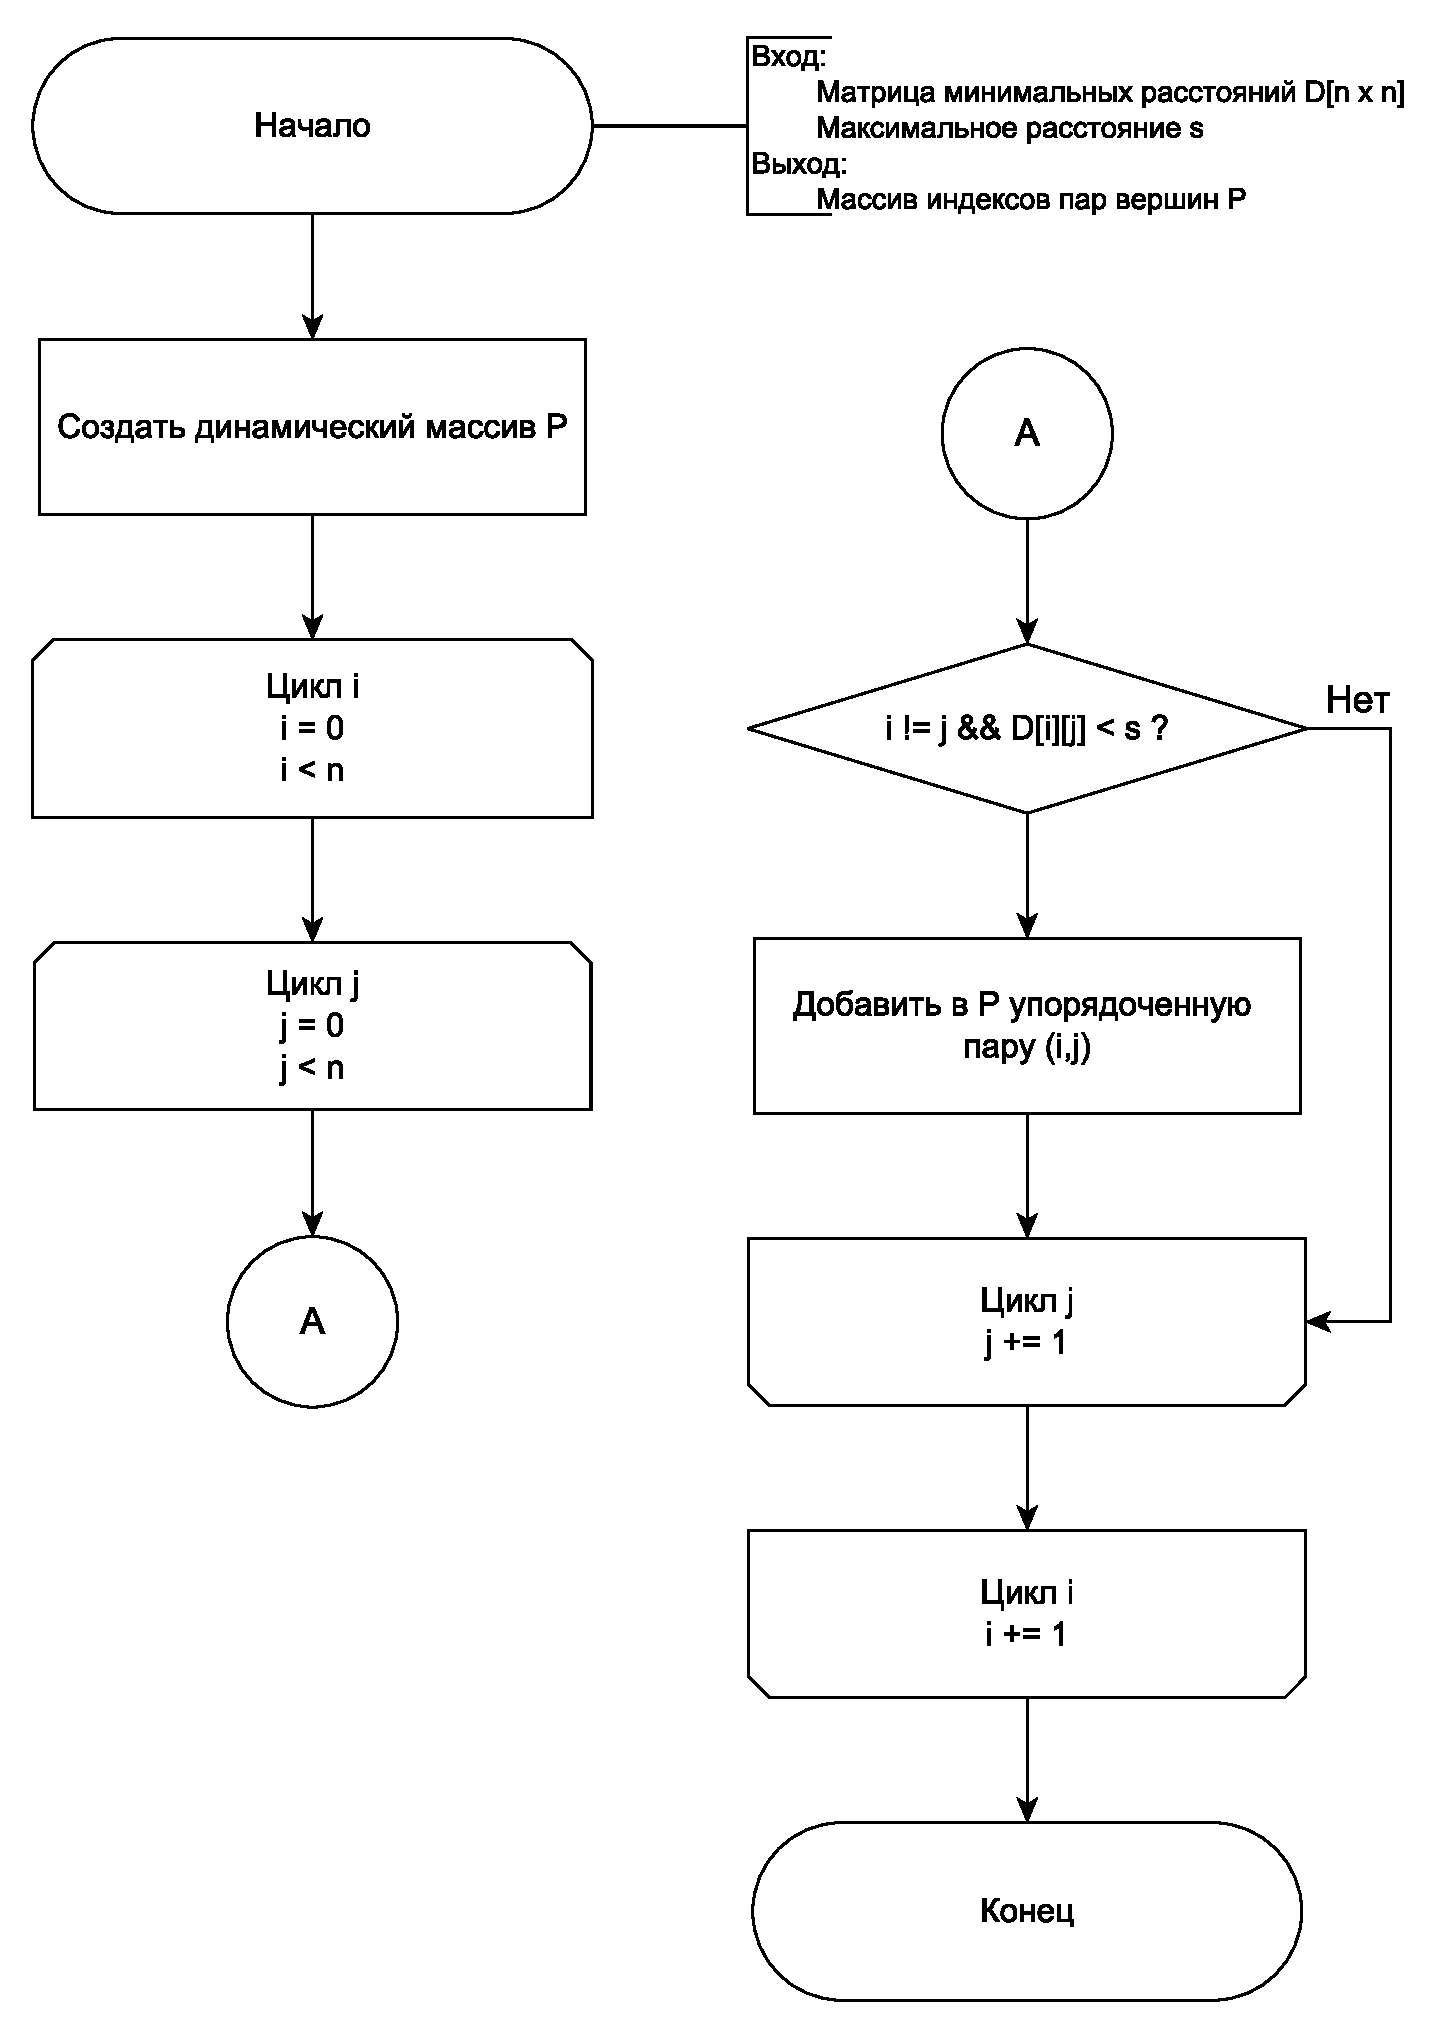
\includegraphics[width=1\textwidth]{images/choose_pairs.pdf}
	\caption{Схема алгоритма выбора пар на расстоянии меньше заданного}
	\label{img:choose_pairs}
\end{figure}

\subsection{Параллельный алгоритм}

На рисунке~\ref{img:parallel_main} приведена схема алгоритма главного потока.

На рисунке~\ref{img:parallel_worker} приведена схема алгоритма рабочего потока, отвечающая за обработку одного блока матрицы кратчайших расстояний.

На рисунке~\ref{img:threadpool} приведены схемы алгоритмов методов пула потоков, необходимых для реализации параллельного алгоритма.

\begin{figure}[H]
	\centering
	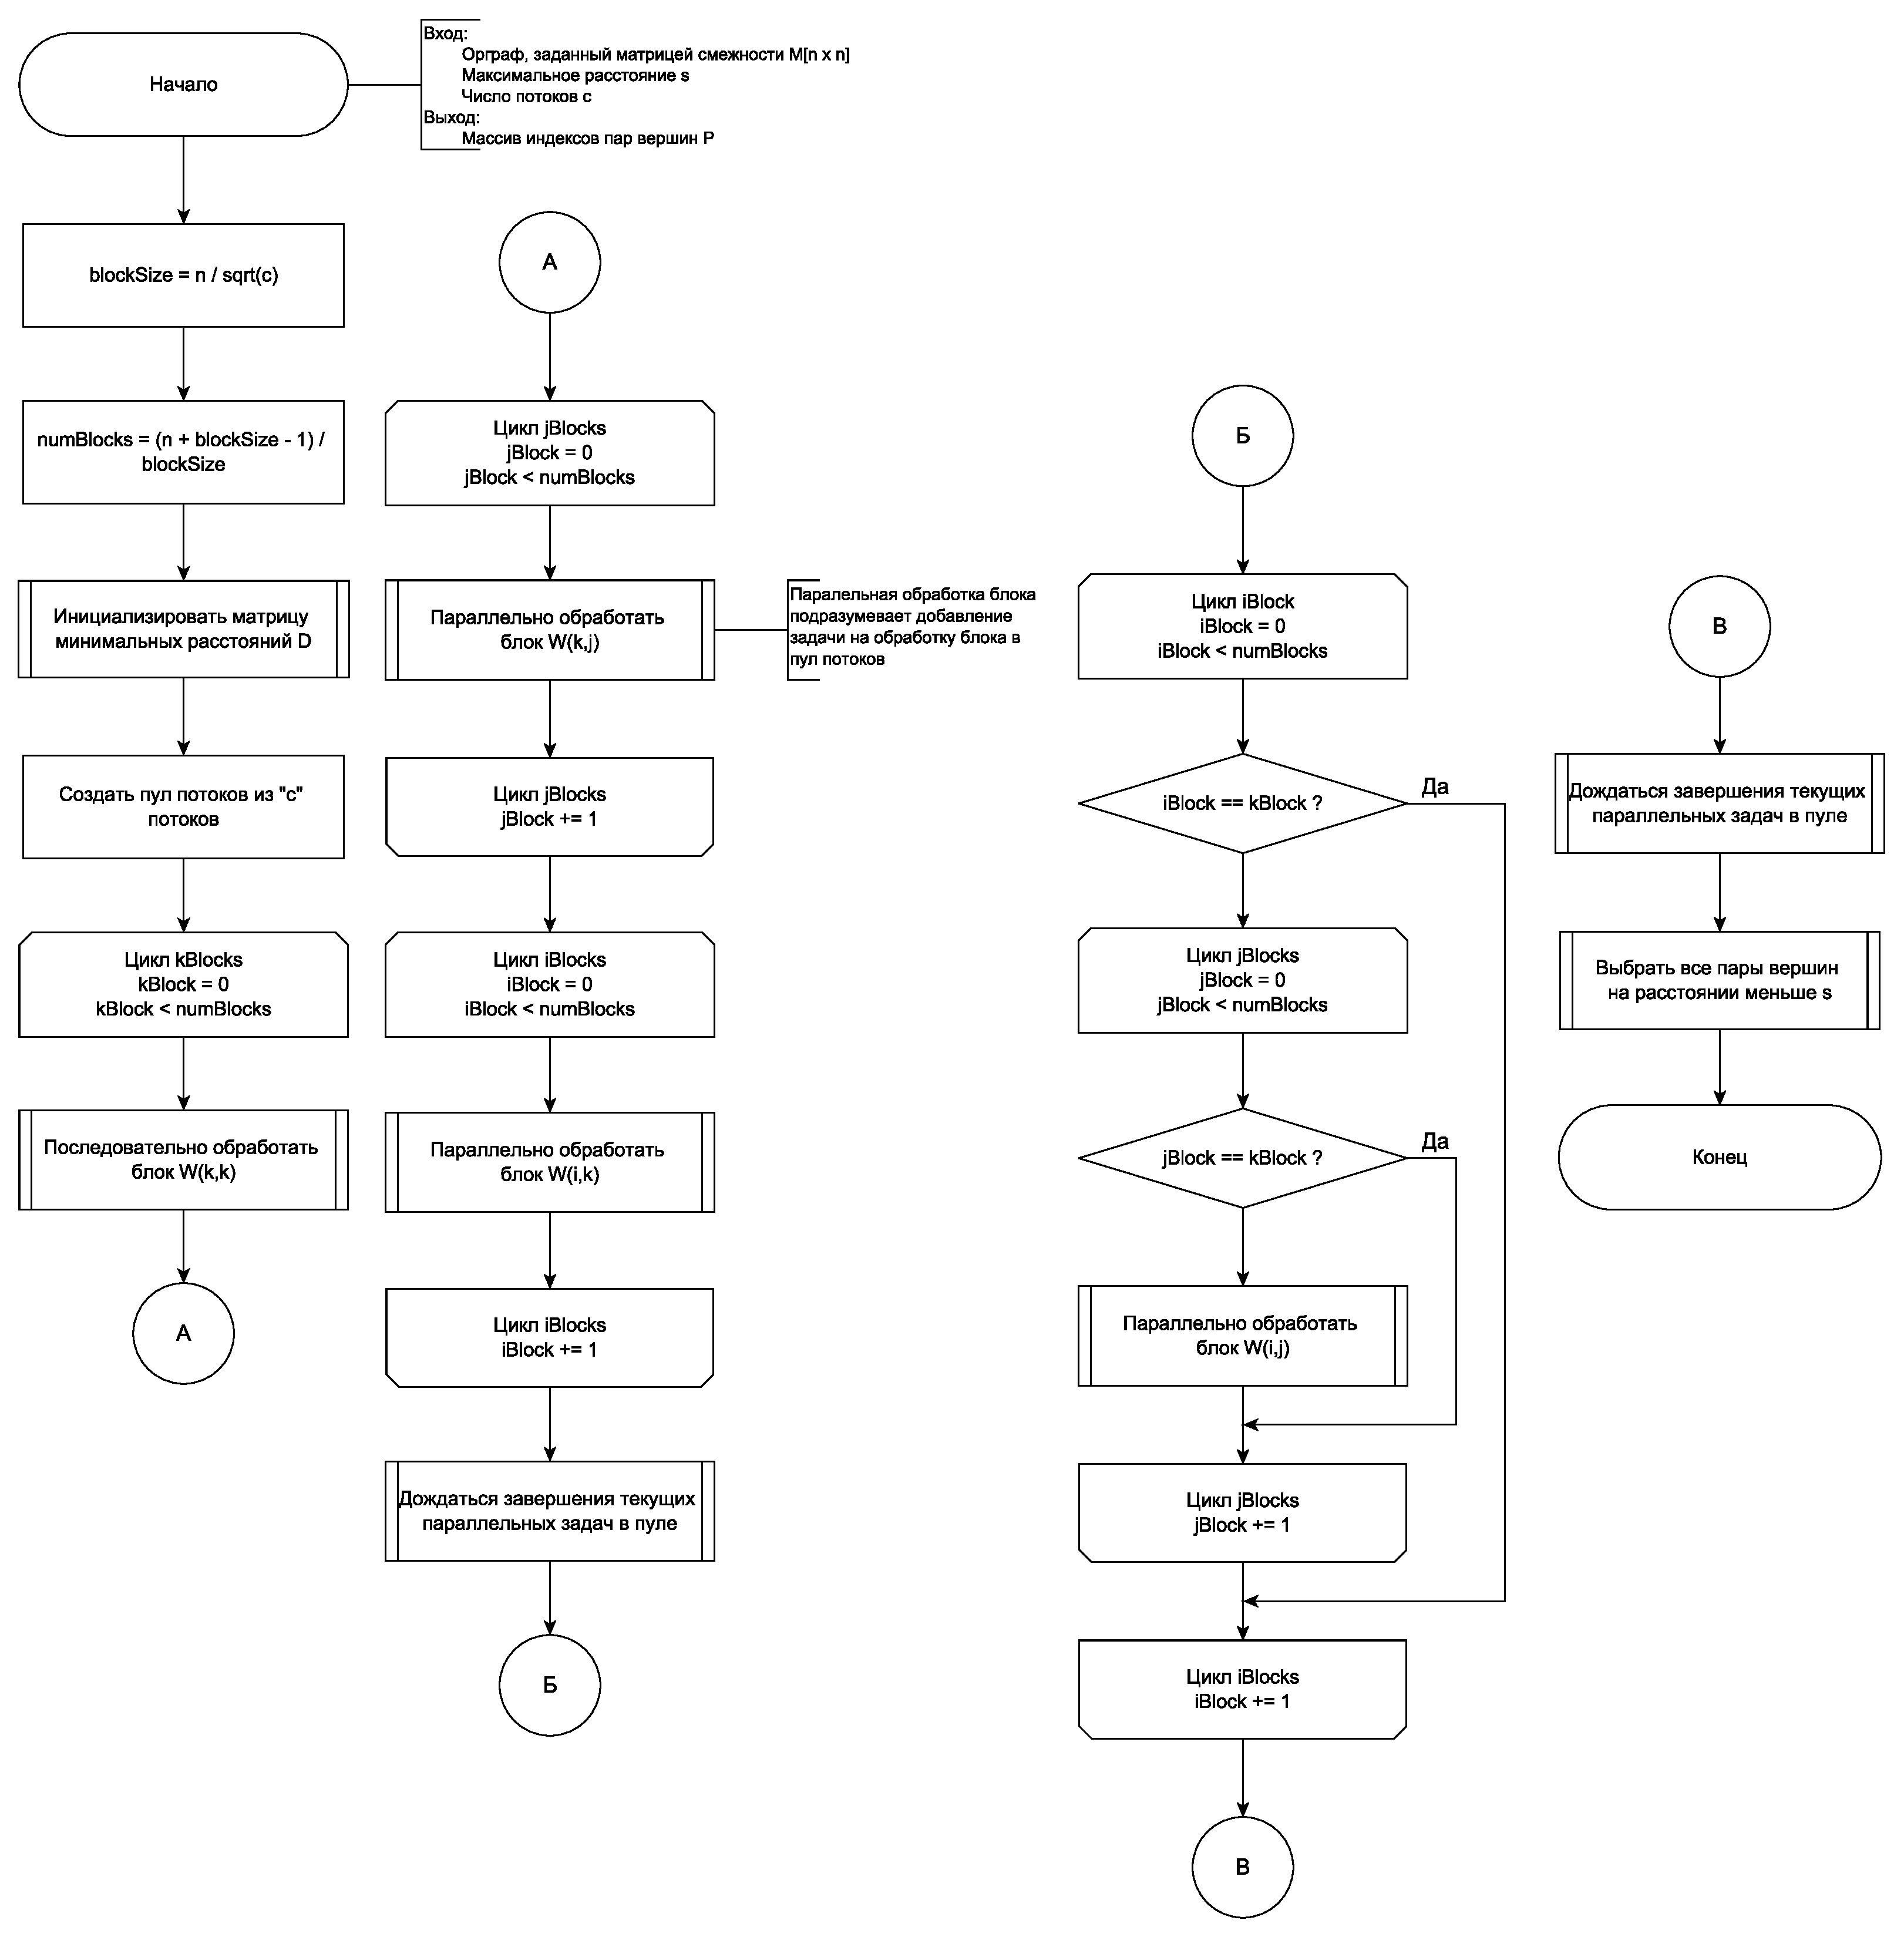
\includegraphics[width=1\textwidth]{images/parallel_main.pdf}
	\caption{Главный поток параллельного алгоритма}
	\label{img:parallel_main}
\end{figure}

\begin{figure}[H]
	\centering
	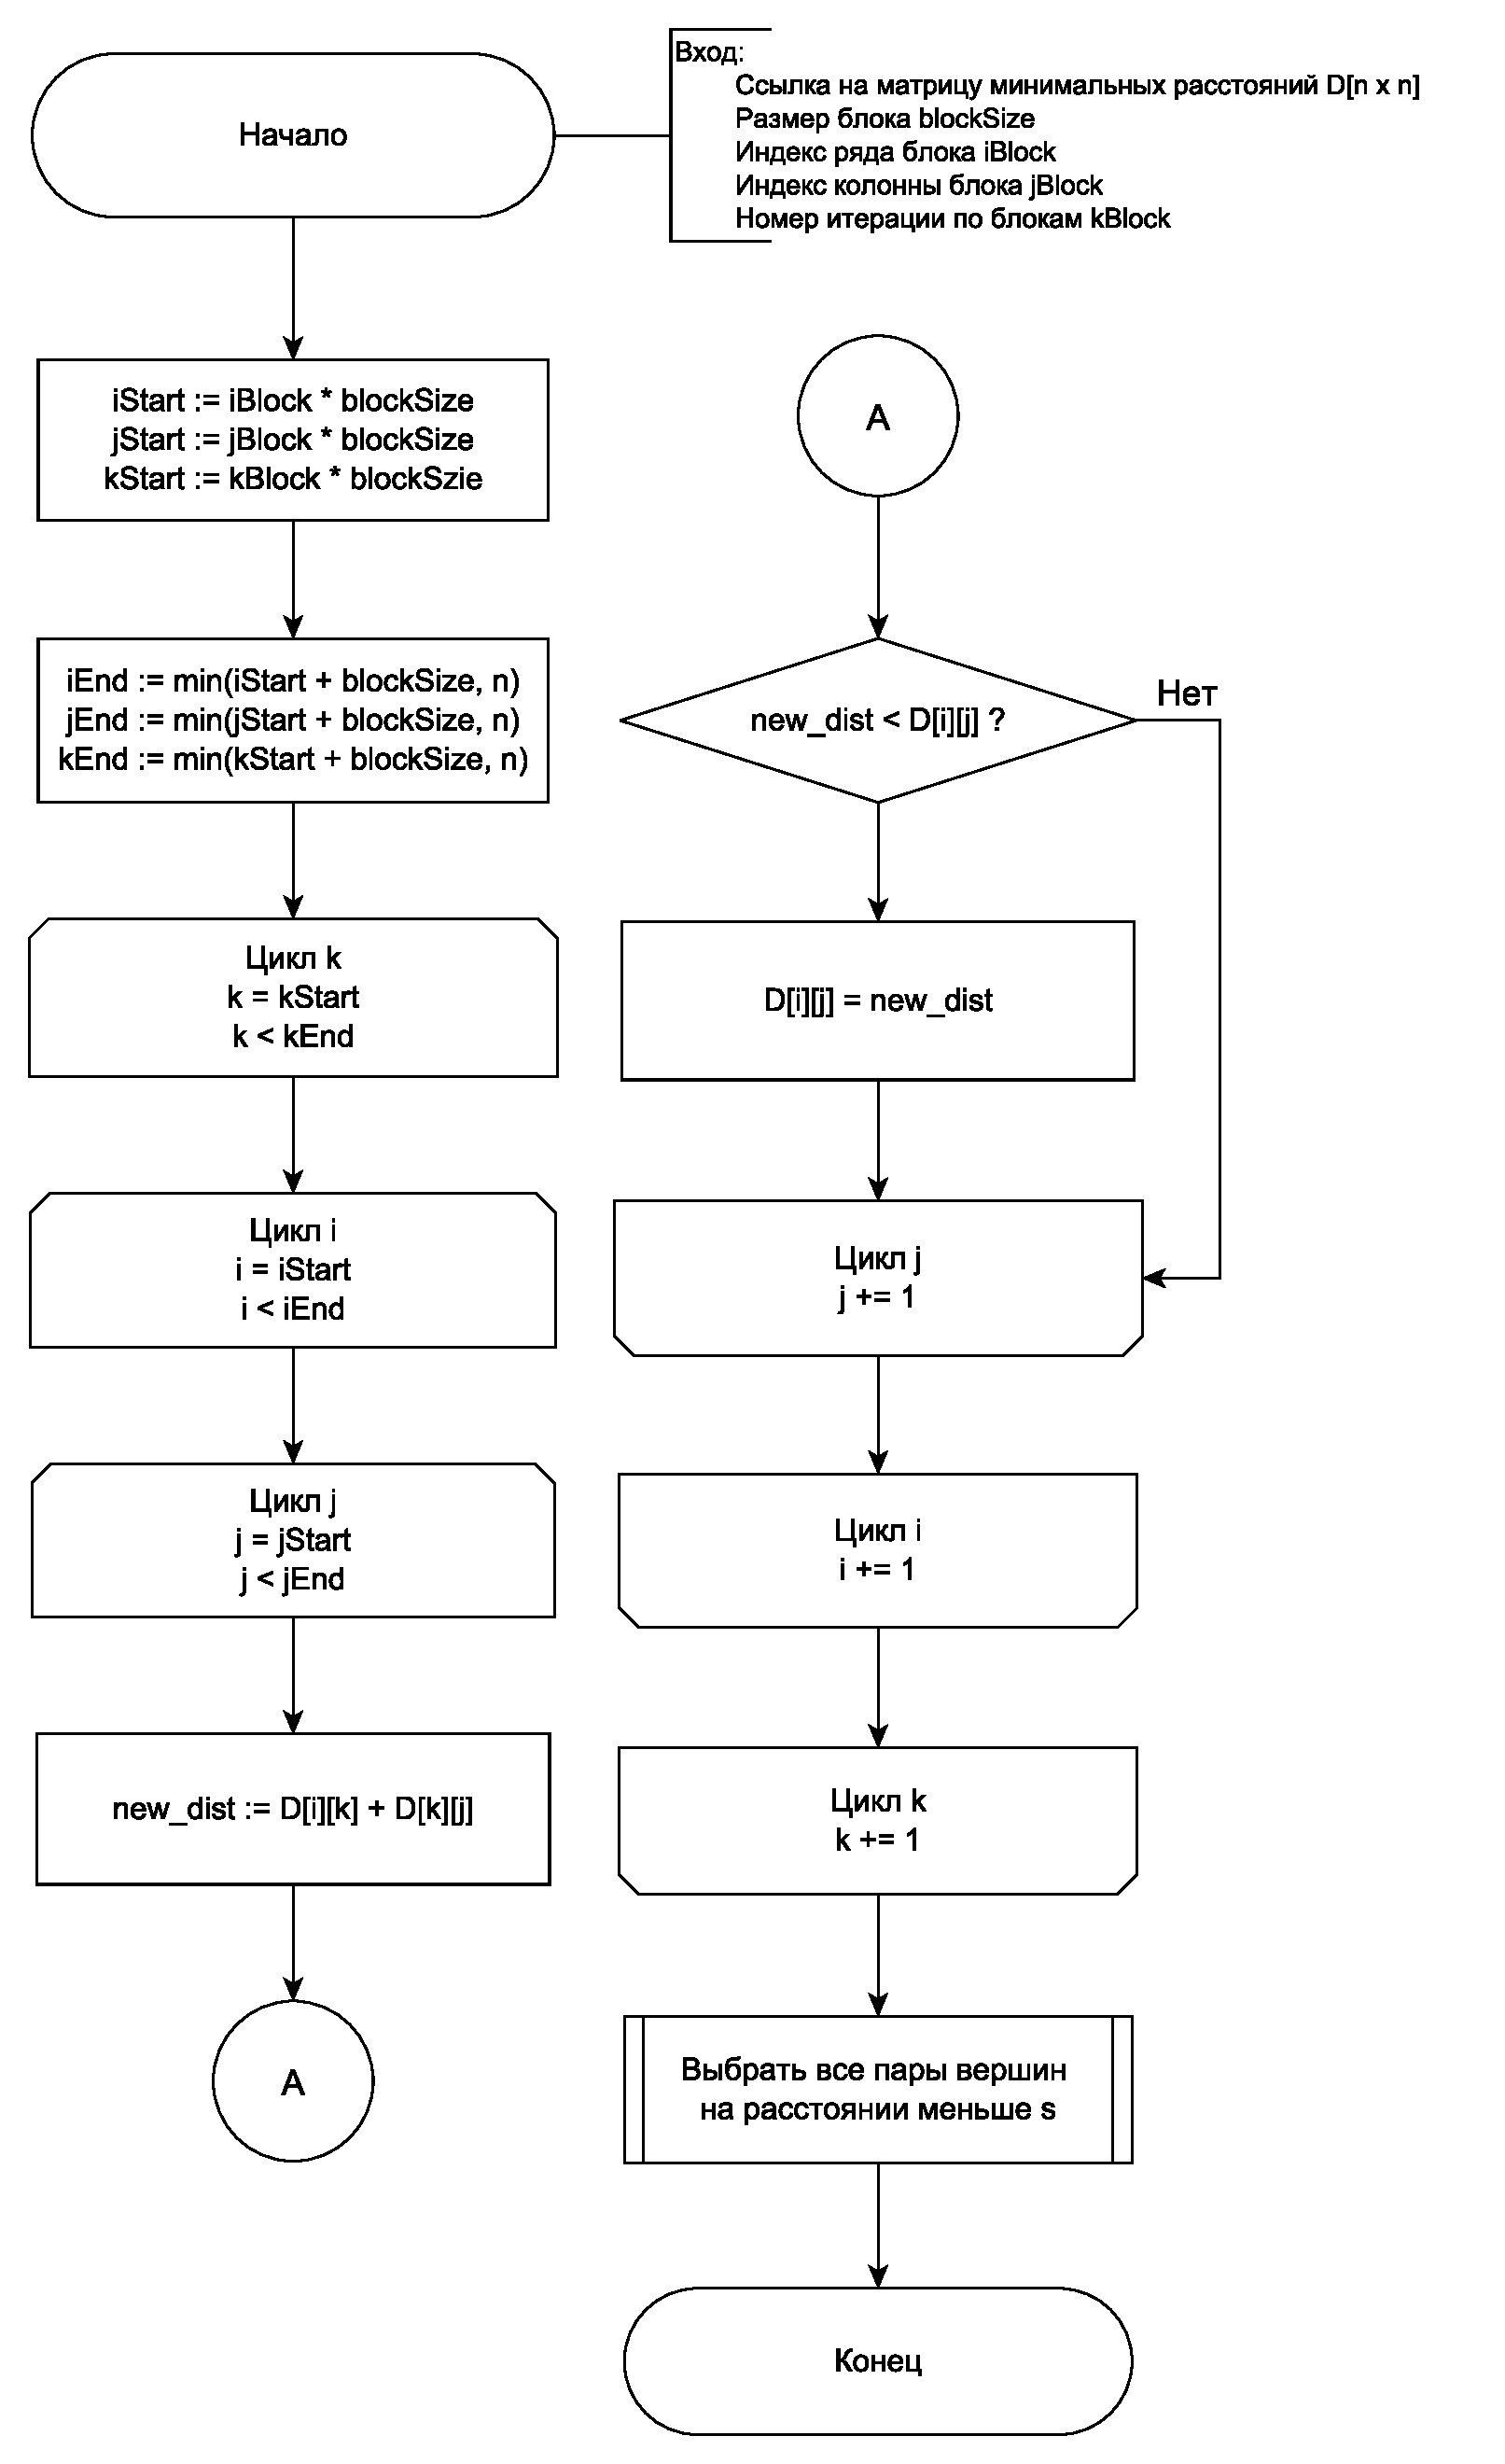
\includegraphics[height=0.9\textheight]{images/parallel_worker.pdf}
	\caption{Рабочий поток параллельного алгоритма --- алгоритм обработки одного блока матрицы минимальных расстояний}
	\label{img:parallel_worker}
\end{figure}

\begin{figure}[H]
	\centering
	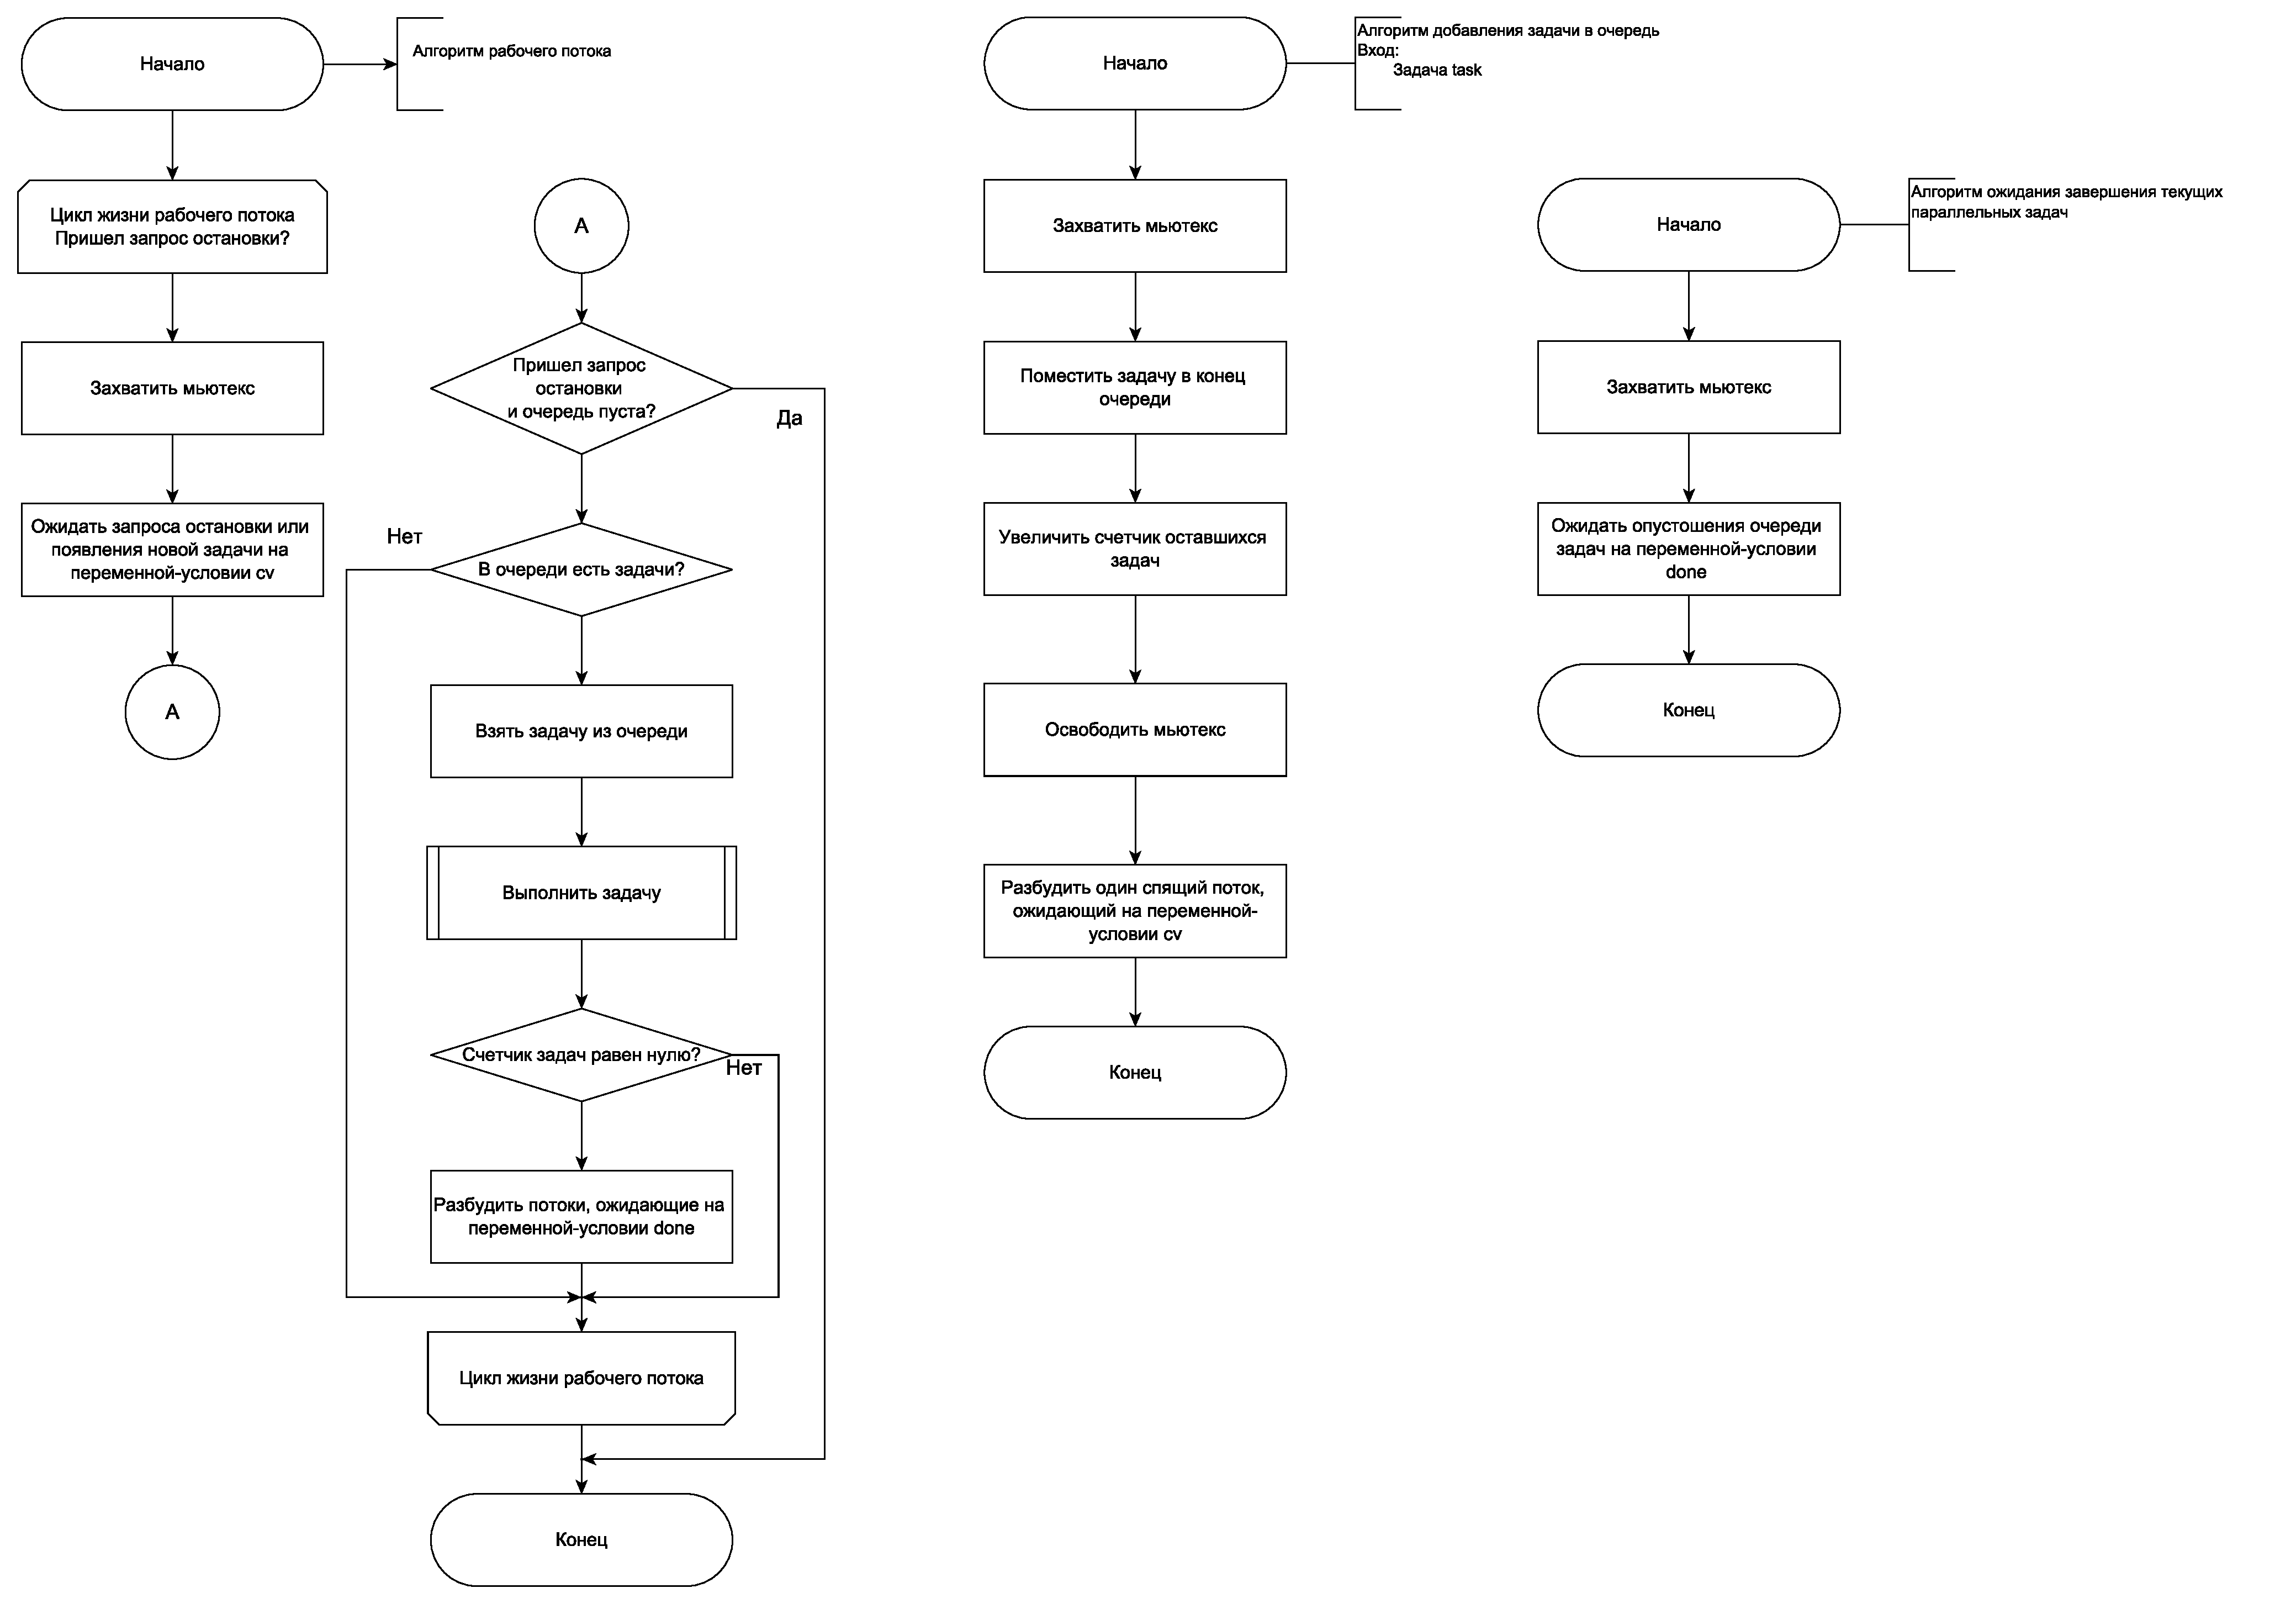
\includegraphics[width=1\textwidth]{images/threadpool.pdf}
	\caption{Схемы алгоритмов методов пула потоков}
	\label{img:threadpool}
\end{figure}

\section*{Вывод}

В данной части были приведены схемы последовательного и параллельного алгоритмов, а также схемы алгоритмов методов пула потоков, необходимые для реализации параллельного алгоритма.

\clearpage
